\documentclass[11pt,a4paper,article,oneside]{memoir}

\usepackage[utf8]{inputenc}
\counterwithout{section}{chapter}

	% Memoir modifications
	\setlength{\parindent}{0em}	% No indent in paragraph start
	\nonzeroparskip
	
	\captionnamefont{\footnotesize\bfseries}
	\captiontitlefont{\footnotesize}
	
	\changecaptionwidth
	\captionwidth{\linewidth}
	
	\setlrmarginsandblock{2.5cm}{2.5cm}{*}
	\setulmarginsandblock{2.5cm}{2.5cm}{*}
	\checkandfixthelayout
	
\usepackage{graphicx}
%\usepackage[font=small]{caption}
%	\captionsetup{width=.9\linewidth, justification=justified, format=plain}

\usepackage{wrapfig}
\usepackage{dirtytalk}
\usepackage{siunitx}
\usepackage{xcolor}

	% Title page
	\aliaspagestyle{title}{empty}
	\pretitle{\begin{center}\vfill \Huge\bfseries {
\includegraphics[width=0.7\linewidth]{title2}}}
		\title{}
		\posttitle{\par\vskip1em{\normalfont\Large\scshape Laser cavity design and analysis\par \normalsize by} \end{center} \Large }
	\author{Julio M. Rodríguez-García}
	\predate{\vfill \centering {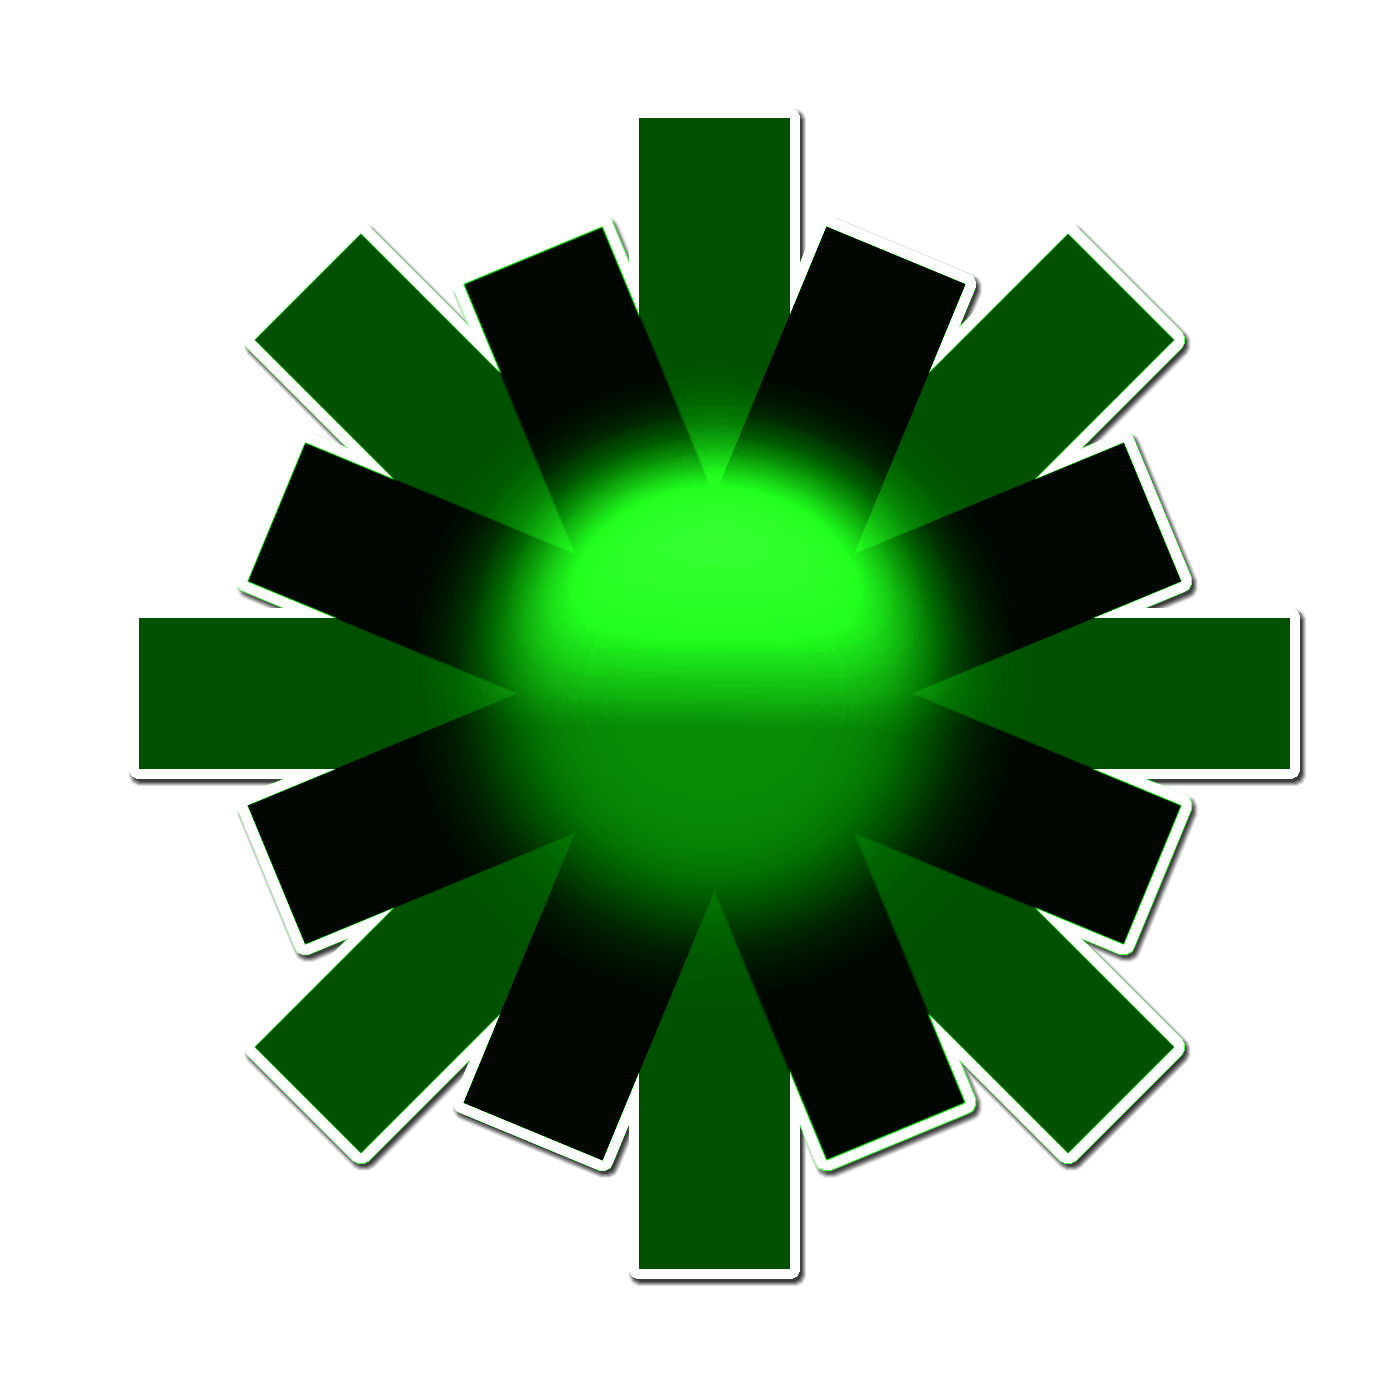
\includegraphics[width=0.25\linewidth]{logo-tg3}} \vfill\begin{center}\large}
		\date{}

% Links
\definecolor{amethyst}{rgb}{0.54, 0.3, 0.89}
\usepackage[colorlinks,linkcolor=blue, urlcolor=amethyst]{hyperref}
\usepackage[nameinlink]{cleveref}

\begin{document}
	\graphicspath{{./Figures/}}
	
	\maketitle
	
	\mainmatter
	\section{Introduction}
	Simcav is a tool for advanced design and analysis of laser cavities. 
	
	It features quick drawing of resonators together with a powerful design calculator for complex cavities. Analysis of beam size and stability is straightforward for both saggital and tangential components. 
	
	The graphical user interface aims for simplicity and easiness of use. 
	
	SimCav is written in Python, a powerful, high-level programming language that emphasizes code readability and simplicity (\say{simple is better than complex, complex is better than complicated}, as expressed in the \href{https://www.python.org/dev/peps/pep-0020/}{Zen of Python}).

	\begin{figure}[h!]
		\centering
		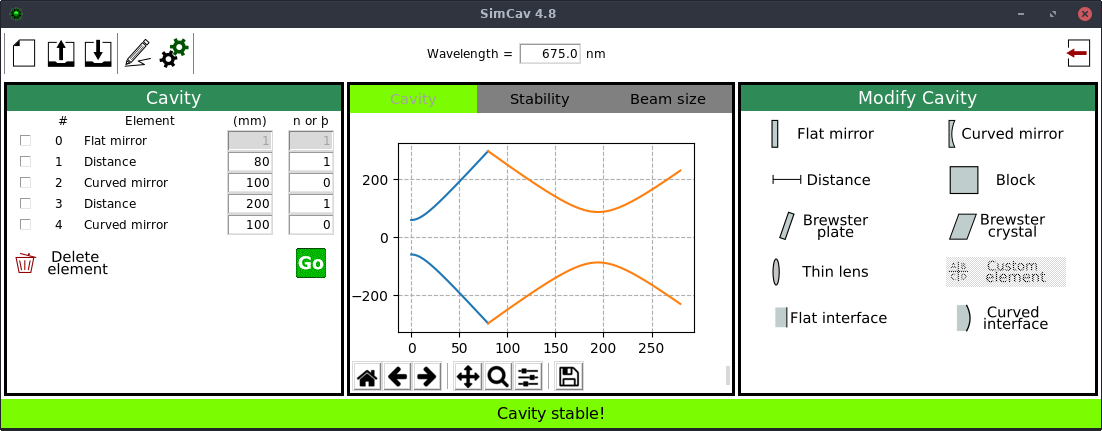
\includegraphics[width=0.8\linewidth]{simcav.png}
		\caption[SimCav]{SimCav interface.}
		\label{fig:simcav}
	\end{figure}

	\section{Features}
	\begin{itemize}
		\item Design calculator:\\
		The built-in calculator can find solutions for cavities based on user-given conditions.
		
		\item Clear interface:\\
		A clear and minimalist interface with everything at hand, with the cavity plot as the central piece.
		
		\item Export the plots:\\
		The plots can be easily saved as image files (e.g. .jpg) for easy sharing, printing, reporting etc.
		
		\item Portable:\\
		No install required, you could keep it in your usb key and run it everywhere you go.
		
		\item Multiplatform:\\
		Use the program or share your designs across multiple operating systems without hassle.
		
		\item Iconographic:\\
		Knowledge of english is not necessary to take full advantage of the software.
		
		\item Open-source:\\
		The source code is available to study or modify and adapt to your needs.
		
		\item Free software:\\
		Respecting your freedom and without charge: no tracking, no ads, \SI{100}{\percent} science.
	\end{itemize}
	
	\newpage
	\section{Layout}
	The interface is built around a central frame used for plotting various diagrams. A toolbar on top provides access to general functions while a status bar at the bottom provides information to the user. The left frame shows the current cavity elements, while the right frame contains SimCav's tools.
	
		\subsection{Toolbar}
		The toolbar displays the common buttons \textit{New, Open} and \textit{Save}. These buttons, respectively, reset Simcav for a new system, open a previously saved system or save the current system. Besides, \textit{Modify cavity} and \textit{Design calculator} are used to display the appropriated tools in the right frame. Centred in the toolbar, the wavelength box is showed, to set the system's wavelength. At the right side, the exit button is present, and works as expected.
		
		\begin{figure}[h!]
			\centering
			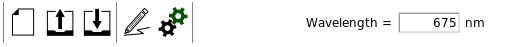
\includegraphics[width=0.7\linewidth]{toolbar.png}
			\caption[Toolbar]{Toolbar.}
			\label{fig:toolbar}
		\end{figure}
		
		% FLOATING TIP
		% SimCav does \textbf{not} prompt for saving.
		
		\subsection{Left frame: Elements}
		\begin{wrapfigure}[10]{R}{0.35\linewidth}
			\normalcaptionwidth
			\vspace{-12pt}	
			\centering
			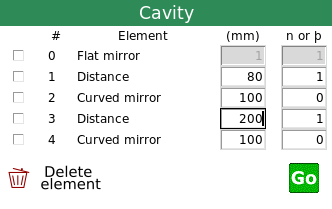
\includegraphics[width=\linewidth]{element-box.png}
			\caption[Element box]{Element box displaying the cavity elements.}
			\label{fig:element-box}
		\end{wrapfigure}

		The element box, initially empty, will show each of the cavity elements in use, in the order they follow within the cavity. They are numbered for unequivocal referencing, since any element may appear repeatedly (e.g. distances). 
		
		Each element is defined by the quantities in the entry boxes next to it. The first one refers to distance or radius of curvature, and the second, to refractive index or tilting angle.
		
		The tick box for each element serves two purposes: it allows for new elements to be inserted above the first ticked element, and it marks elements for deletion (can be various at the same time). To delete elements simply tick their boxes and click the \textit{Delete element} button.
		
		Finally, the \textbf{Go} button instructs SimCav to draw the cavity as defined by the current elements. If the cavity is not stable, or there are other issues, a message will appear in the status bar.
		
		% FLOATING TIP
		% The entries can be navigated with the \textit{TAB} key, and \textit{Enter} key is linked to the \textbf{Go} button.
		
		\newpage
		\subsection{Central frame: Plots}
		The centre of the layout displays several plots for cavity analysis. 
		
		\textit{Cavity} represents the whole resonator, with different colours for each optical element. Elements without length dimension, such as mirrors, are not represented but can be inferred by the change in the beam geometry and the change in colour. The horizontal coordinate represents the total length in millimetres, starting at the first element, and the vertical coordinate represents the beam size in micrometres. The positive and negative section of the Y-axis stands for the tangential and saggital components of the beam (and will be the same in each plot).
				
		\begin{figure}[h!]
			\centering
			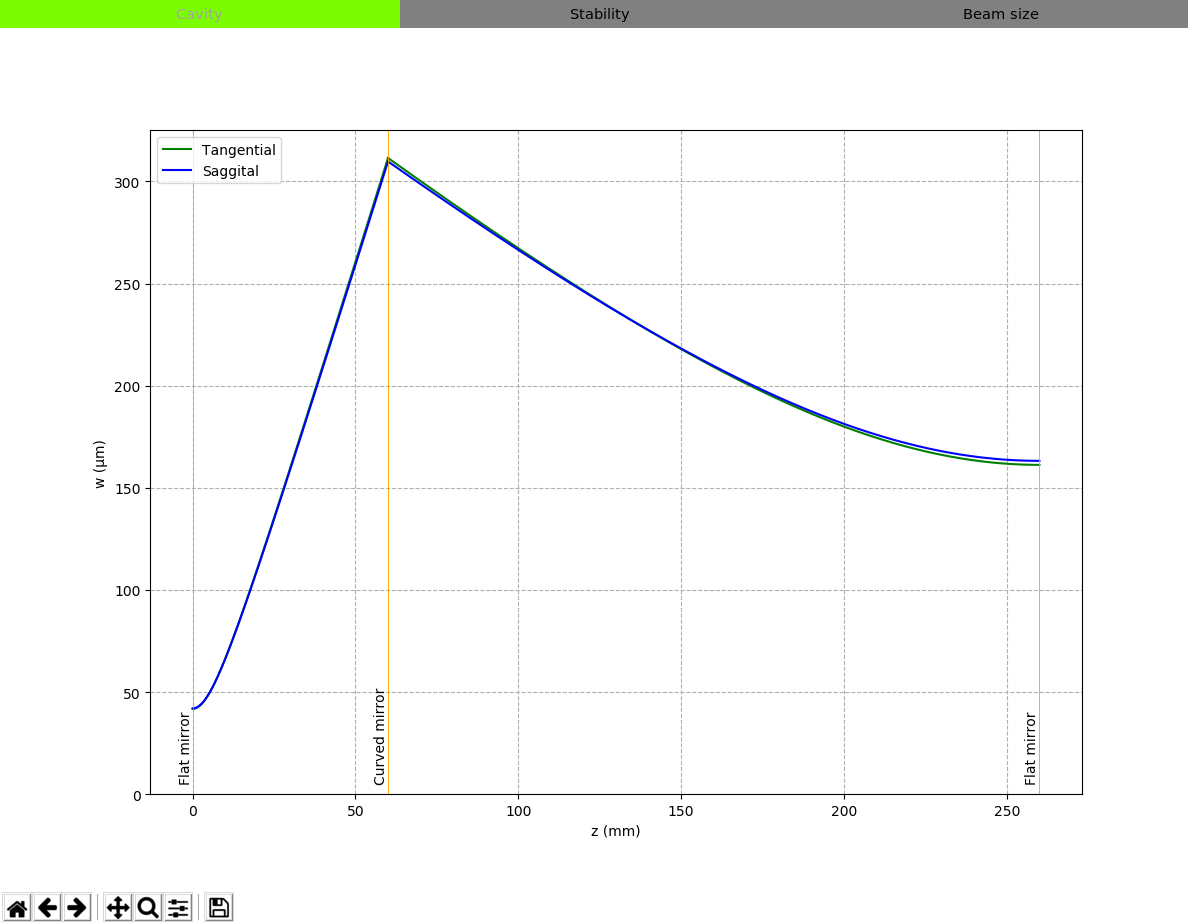
\includegraphics[width=0.8\linewidth]{central-frame.png}
			\caption[Cavity frame]{Central frame displaying the cavity. In this case, we can see a 3-mirror cavity, with the mirrors separated 80 mm and 200 mm.}
			\label{fig:central-frame}
		\end{figure}
	
		\textit{Stability} represents the stability of the resonator in function of the variation of a chosen element. The element to vary and the variation range can be set with the top menus, as seen in \cref{fig:stability-frame}.
		
		\begin{figure}[h!]
			\centering
			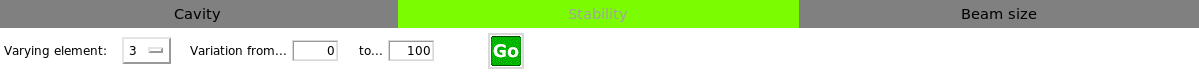
\includegraphics[width=0.8\linewidth]{stability-crop.png}
			\caption[Stability frame]{Top region of stability frame. Stability can be calculated for the variation of any of the cavity elements.}
			\label{fig:stability-frame}
		\end{figure}
	
		\textit{Beam size} represents the beam size at any given non-length-dimension element for the variation of any of the cavity elements. Said elements can be chosen with corresponding dropdown menus, and the variation range set with the entry boxes.
		
		\begin{figure}[h!]
			\centering
			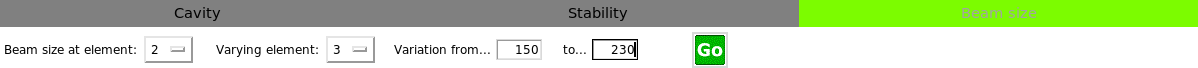
\includegraphics[width=0.8\linewidth]{beamsize-crop.png}
			\caption[Beam size frame]{Top region of stability frame. Stability can be calculated for the variation of any of the cavity elements.}
			\label{fig:beamsize-frame}
		\end{figure}
				
		\newpage
		\subsection{Right frame: Tools}
		
			\subsubsection{Modify cavity}
			\begin{wrapfigure}[10]{R}{0.4\linewidth}
				\normalcaptionwidth
				\vspace{-12pt}
				\centering
				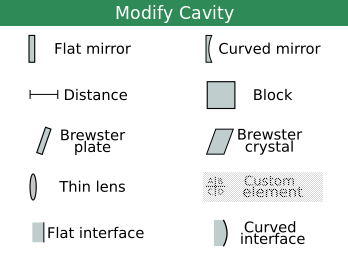
\includegraphics[width=\linewidth]{modify-box.png}
				\caption[Modify cavity]{Modifying cavity elements.}
				\label{fig:modify-box}
			\end{wrapfigure}
		
			This section presents the user with all the available elements. Simply clicking on any will add it to the cavity, and it will appear in the \textit{element box} (left frame). Since reordering is not implemented at the moment, the user is advised to click on the elements in the order they will follow in the built cavity (for speed). The given default values can be later changed.
			
			This toolbox can be accessed any time by clicking the \textit{Modify cavity} button in the toolbar. Any new cavity starts with this box conveniently opened.
		
			\subsubsection{Design calculator}
			SimCav features a design calculator to find a cavity suitable for the user needs. This toolbox displays the controls required to configure and launch such calculator.
			
			\begin{wrapfigure}[15]{R}{0.4\linewidth}
				\normalcaptionwidth
				\vspace{-12pt}
				\centering
				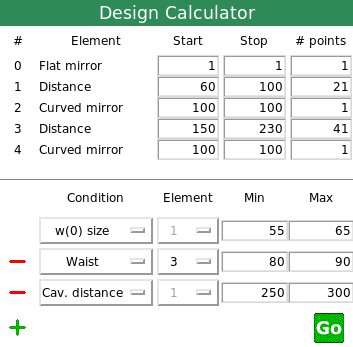
\includegraphics[width=\linewidth]{design-box.png}
				\caption[Desing calculator]{Design calculator.}
				\label{fig:design-box}
			\end{wrapfigure}
			
			In the top half, the cavity elements are displayed together with their position in the cavity, followed by three entry boxes. These boxes refer to the variation of the elements for calculation purposes. In order they represent the start and finish of the variation, and the number of points to study. Any number of elements can be modified at the same time, at the cost of increased calculation time.
						
			The bottom half displays the conditions that must be fulfilled to find a solution. It features a dropdown menu to choose the condition and the element it applies to, together with the minimum and maximum threshold values. Not every condition can be applied to every optical element.
			
			The available conditions are w(0) ---beam size at $z=0$, i.e. at the beginning of the cavity---, \textit{Waist} ---waist at an extended element--- and \textit{Cav. distance} ---setting a range of total distances acceptable for the whole cavity---. The user may choose as many conditions as needed, using the \textit{add} (and \textit{delete}) buttons provided.
			
			This toolbox can be displayed by pressing the \textit{Design calculator} button in the toolbar.
		
		\subsection{Results window}
		The \textit{results} window displays, in rows, each system configuration that fulfils the given conditions, together with the stability of such system and the actual values of the chosen conditions. It is possible to click on any condition for the corresponding system configuration to be automatically imported and displayed.
		
		\begin{figure}[h!]
			\centering
			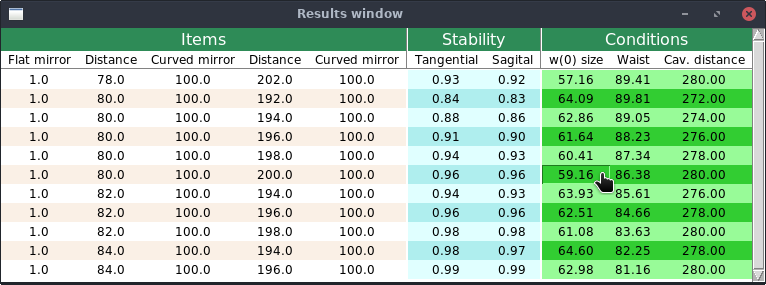
\includegraphics[width=0.7\linewidth]{results-window.png}
			\caption[Results window]{Design calculation results shown in a separate window.}
			\label{fig:results}
		\end{figure}
		
		The results of the design calculation are shown in a separate window so several calculations can be run without losing the previous results.
	
	\newpage
	\section{Optical elements}
	SimCav provides the following optical elements.
	
	\begin{itemize}
		\item Flat mirror: No need of extra parameters.
		
		\item Curved mirror: First parameter: curvature radius (in millimetres). Second parameter: Tilting angle from the vertical plane (in degrees).
		
		\item Distance: This element corresponds to free space. First parameter: distance in millimetres. Second parameter: refractive index. Attention: this is the refractive index of the medium the cavity is immersed in. Therefore it is typically air, and its value is 1 by default.
		
		\item Block: Element to model intracavity crystals or other elements with different refractive index than that of the free space. It includes modelling of input and output interfaces (making it different from Distance element).
		
		\item Brewster plate and Brewster crystal: Both elements correspond to crystals at Brewster's angle from the optical axis. Brewster plate is a rectangular prism while Brewster crystal is a rectangular rhombohedrum. Longitudinal faces of the Brewster crystal are parallel to the ptical axis of the cavity. First parameter: length of the element. Second parameter: refractive index.
		
		\item Thin lens: First parameter: focal length. Second parameter: Tilting angle from the vertical plane.
		
		\item Custom element: Allows the user to define a custom element with the 4 ABCD parameters. This feature is experimental, and at the moment, disabled.
		
		\item Flat and curved interfaces: First parameter is the radius of curvature (disabled in the case of	flat interface). Second parameter: refraction index of the medium after the interface. Please note that length-dimension elements should have the correct refractive index set.
	\end{itemize}
	
%	\section{Advanced tricks}
%	Set default wavelength.
	\newpage
	\section{Running SimCav}
	SimCav is portable and therefore it does not install in the system. Simply download the appropriate binary from the website and run it.
	
	If you prefer to run SimCav from source, download the code (if using git you can clone it directly: \say{git clone https://github.com/simcav/simcav}) and run the \textit{simcav\_main.py} file with Python 3. SimCav does not support Python 2. 
	
	The \textit{matplotlib} library did a non-backwards-compatible change in the version 1.5, so if using any older version SimCav will not work. Please always ensure to update your system!
	
	The releases are digitally signed with the SimCav key (public key available on the website). Once extracted, it is possible to use GPG or similar to verify the download (\say{gpg --verify SimCav.asc}).
		
	
\end{document}